
% This work is licensed under the Creative Commons Attribution-Share Alike 2.0 France License.
% To view a copy of this license, visit http://creativecommons.org/licenses/by-sa/2.0/fr/legalcode
% or send a letter to Creative Commons, 171 Second Street, Suite 300, San Francisco, California, 94105, USA.



\chapter{Un court chapitre à propos des fichiers}\label{ch:ashortchapteraboutfiles}
\section{Sauvegarde des programmes}

Vous savez déjà probablement ce qu'est un fichier ( \emph{file} en anglais pour l'informatique).
Dans votre classe vous avez probablement des fiches --- par exemple de lecture, de botanique--- qui sont réunies ensembles au sein de fichiers. Ces fichiers sont réunis dans des boites pour faciliter leur utilisation.

C'est assez similaires en informatique, nous mettons les informations dans des fichiers que nous rangeons dans des répertoires (appelés aussi dossiers), la \autoref{fig:Files11_directory_hierarchy} montre cette organisation.

\begin{figure}[h!]
\centering
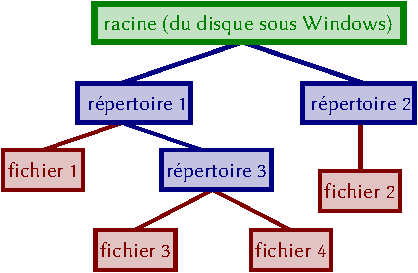
\includegraphics[scale=1]{images/Files11_directory_hierarchy.pdf}
\caption{Organisation des fichiers et des répertoires}\label{fig:Files11_directory_hierarchy}
\end{figure}


Rappelez-vous au premier chapitre nous avions créé un fichier «~\texttt{bonjour.py}~» et nous ne pouvions pas voir le résultat de l'exécution de programme.

Nous allons maintenant voir comment utiliser ce type de fichier.
Premièrement cliquez avec le bouton droit de la souris sur le fichier bonjour.py et choisissez «~\texttt{éditer avec IDLE}~» comme sur la \autoref{fig:edit_idle}.
\begin{figure}[h!]
\centering
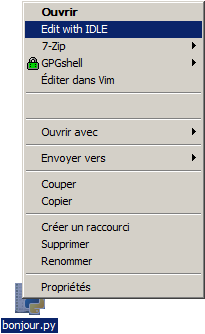
\includegraphics[scale=0.5]{images/edit_idle.png} 
\caption{Édition avec IDLE}
\label{fig:edit_idle}
\end{figure}

Deux fenêtres s'ouvrent alors: l'éditeur et le shell comme montrés sur 
la \autoref{fig:ouvert_idle}.
\begin{figure}[h!]
\centering
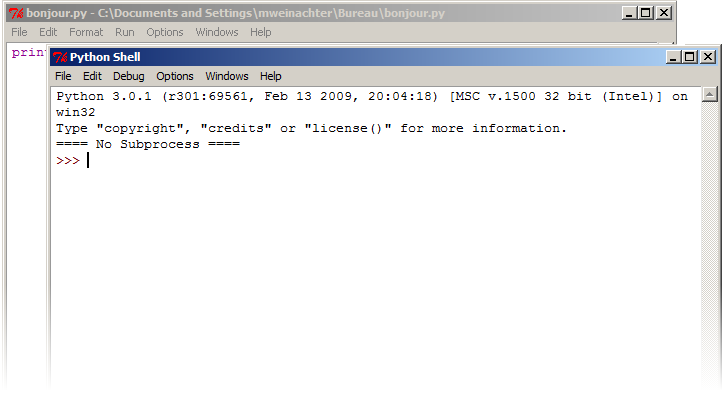
\includegraphics[scale=0.5]{images/ouvert_idle.png} 
\caption{Fenêtres d'IDLE}
\label{fig:ouvert_idle}
\end{figure}

Selon vos préférences vous pouvez afficher l'une ou l'autre des fenêtres . \\

\emph{En tant que livre je préfère une présentation de type une page à gauche et
 une page à droite. Pour ce faire je clique droit sur la barre des tâches et je choisis mosaïque verticale.}\\

Comme vous le voyez, le code que vous aviez entré est affiché dans la fenêtre «~Bonjour.py~». Sélectionnez cette fenêtre puis appuyez sur la touche «~\texttt{F5}~» ou cliquez sur «~\texttt{Run}~» (courir en anglais normal, exécuter en informatique) puis «~\texttt{run module}~». Le résultat s'affiche dans le shell.

Comme vous le voyez vous pouvez éditer, sauvegarder et réutiliser le code que vous réalisez.

Modifier le code comme suit: 

\begin{Verbatim}[frame=single,rulecolor=\color{mbleu}, label=à taper]
import sys

print("Bonjour le monde")
sys.stdin.readline()
\end{Verbatim}

Puis lancez le avec la touche «~\texttt{F5}~» l'éditeur va vous demander de sauvegarder le fichier pour pouvoir l'exécuter, répondez oui car c'est ce que nous voulons. Le programme s'exécute et attend que vous appuyez sur entrée. Plus intéressant vous pouvez double-cliquer sur le fichier «~\texttt{bonjour.py}~». Le message s'affiche et reste affiché. \\

\emph{Vous pouvez, si vous le souhaitez, compléter ce programme et le montrer à votre entourage. Par exemple, vous pouvez poser une question et composer une réponse à partir de celle-ci.}\\

\begin{Verbatim}[frame=single,rulecolor=\color{mbleu}, label=à taper]
import sys

print("Bonjour, quel est votre nom ?")
nom=sys.stdin.readline()[:-1]
print("Bonjour, %s. Comment allez vous ?" % nom)
état=sys.stdin.readline()[:-1]
print("Moi aussi je vais %s." % état)
print("Appuyez sur entrée pour quitter.")
sys.stdin.readline()
\end{Verbatim}

Pour information, le «~\texttt{[:-1]}~»  indique à Python de prendre tous les caractère rentrés moins un. Le dernier caractère correspond au retour à la ligne créé par la touche entrée.


\section{Si ça ne passe pas la fenêtre, passons par le soupirail}
Microsoft a décidé au cours des évolutions de son système d'exploitation de changer les endroits (répertoires) utilisés pour le bureau (ce qui affiché une fois l'ordinateur démarré) et les documents. Ces répertoires dont le nom était traduit, ont maintenant toujours des noms anglais.

De plus certains chemins simples d'accès comme «~\Verb+C:\+~» ne sont plus toujours accessibles pour des raisons de sécurité.

Il existe des modules qui permettent à Python de connaitre le chemin vers votre bureau ou votre répertoire personnel sans programmation mais ils nécessiteraient une installation supplémentaire. Or nous ne voulons pas déranger vos parents (ou assimilés) à nouveau... Ils sont tellement bien tranquilles sur le canapé.

Nous pourrions, sans programmation, créer un raccourci sur le bureau pour que vous puissiez accéder facilement à votre répertoire personnel qui contient le «~\texttt{bureau}~»  et «~\texttt{mes documents}~». Cette solution est présentée pour information \autoref{fig:etapesra} page \pageref{fig:etapesra}. Mais cette solution est assez longue et finalement assez éloignée de mon sujet.

\begin{figure}[H]
\centering
%\subfigure[Caption of subfigure 1]{
%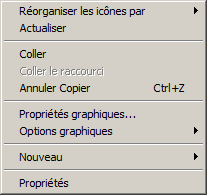
\includegraphics[scale=0.5]{images/clickdb.png}
%\label{fig:subfig1}
%}
\subfigure[Clic droit sur le bureau]{
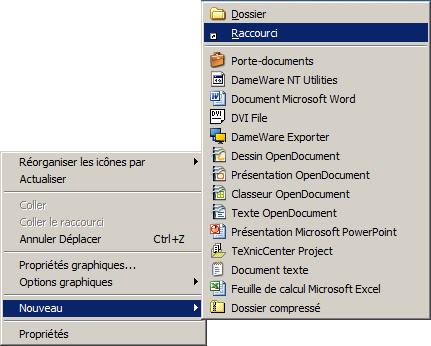
\includegraphics[scale=0.5]{images/nouvra.png}
\label{fig:nouvra}
}
\subfigure[Entrée de «~\texttt{\%userprofile\%}~»]{
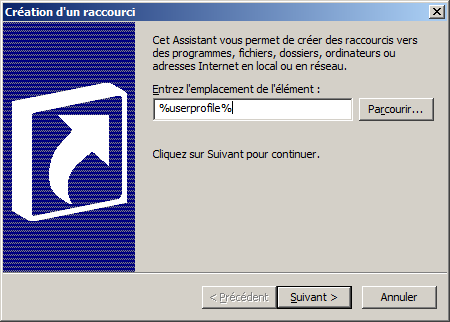
\includegraphics[scale=0.5]{images/creara.png}
\label{fig:creara}
}
\subfigure[Nom du raccourci par défaut]{
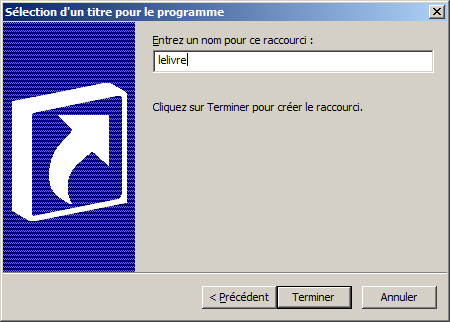
\includegraphics[scale=0.5]{images/comptera.png}
\label{fig:comptera}
}
\subfigure[Entrée de «~\texttt{maison}~»]{
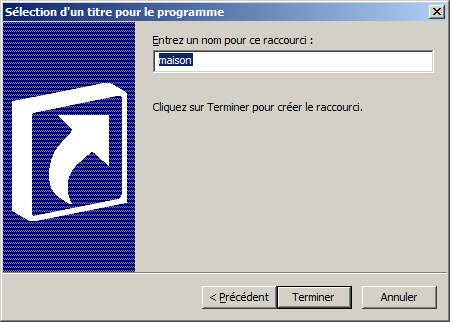
\includegraphics[scale=0.5]{images/maison1.png}
\label{fig:maison1}
}

\subfigure[Le raccourci sur le bureau]{
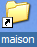
\includegraphics[trim = -40mm 0mm -40mm 0mm, clip,scale=1]{images/maison2.png}
\label{fig:maison2}
}
\caption{Étapes de la création d'un raccourci vers le répertoire personnel}
\label{fig:etapesra}
\end{figure}


C'est pourquoi je vous propose de retrouver le chemin de votre bureau avec Python.
Dans le shell ou dans l'éditeur, faites «~\texttt{Ctrl+N}~» ou «~\texttt{file}~» puis   
«~\texttt{New Window}~», une nouvelle fenêtre de l'éditeur s'ouvre alors.

Vous pouvez identifier la variante du système d'exploitation que vous utilisez:
\begin{Verbatim}[frame=single,rulecolor=\color{mbleu}, label=à taper]
import os,platform

print(platform.release())
print(os.environ['USERPROFILE'])
\end{Verbatim}

Après avoir tapé F5 et sauvegardé le fichier (avec l'extension «~\texttt{.py}~»)  vous devriez avoir quelque chose comme:

\begin{Verbatim}[frame=single,rulecolor=\color{gray}, label=résultat]
XP
C:\Documents and Settings\lelivre
\end{Verbatim}

Nous venons d'obtenir la version de Windows et le chemin vers votre répertoire personnel.
Utilisons alors ces données pour avoir le chemin vers votre bureau:

\begin{Verbatim}[frame=single,rulecolor=\color{mbleu}, label=à taper]
import os,platform

def chemin_bureau() :
    if platform.release()=='XP' :
        return os.path.join(os.environ['USERPROFILE'],"Bureau")
    else :
        return os.path.join(os.environ['USERPROFILE'],"Desktop")
\end{Verbatim}

Exécutons ce module: il ne se passe rien! C'est parce que le fichier que nous venons de créer est un module qui introduit une fonction «~\texttt{chemin\_bureau()}~» mais ne la lance pas. Nous devons modifier légèrement le fichier pour lancer la fonction et, par exemple, afficher le résultat:

\begin{Verbatim}[frame=single,rulecolor=\color{mbleu}, label=à taper]
import os,platform

def chemin_bureau() :
    if platform.release()=='XP' :
        return os.path.join(os.environ['USERPROFILE'],"Bureau")
    else :
        return os.path.join(os.environ['USERPROFILE'],"Desktop")
    
print(chemin_bureau())
\end{Verbatim}

Le résultat que vous devez obtenir doit ressembler à ce qui suit:

\begin{Verbatim}[frame=single,rulecolor=\color{gray}, label=résultat]
C:\Documents and Settings\lelivre\Bureau
\end{Verbatim}

Notez que mon nom d'utilisateur est «~\texttt{lelivre}~», le votre est sûrement votre prénom.

Examinons ce que Python vient de faire. En premier Python importe deux modules «~\texttt{os}~» et «~\texttt{platform}~». Le module «~\texttt{platform}~» apporte des informations sur la plateforme qui sert à lancer les programmes (version du système d'exploitation par exemple). Le module «~\texttt{os}~» apporte une interface pour communiquer avec le système d'exploitation, \emph{operating system} en anglais.

Puis une fonction «~\texttt{chemin\_bureau}~» est créée qui ne prend aucun paramètre en entrée. Python regarde alors le type de Windows utilisé puis selon le résultat retourne le chemin vers le bureau au format approprié en joignant le chemin vers votre répertoire personnel et la chaîne utilisé par votre version de Windows pour identifier le bureau.

Enfin nous avons indiqué à Python que nous voulions qu'il affiche avec «~\texttt{print}~» le résultat de la commande «~\texttt{chemin\_bureau}~».

Dans un programme plus important on crée généralement une fonction «~\texttt{main}~» qui sera exécutée en premier. Cette convention facilite la lecture d'un programme par d'autres personnes.

\section{Un peu de lecture, maintenant?}
Quand Python est installé sur votre ordinateur, un tas de fonctions et de modules sont aussi installés. Certaines fonctions sont disponibles par défaut. La fonction «~\texttt{range}~» que nous avons déjà vue est de ce type. nous allons maintenant regarder la fonction «~\texttt{file}~» que nous n'avons pas encore utilisée.

Pour voir comment les fichiers sont utilisés ouvrez le bloc-notes, tapez quelques lignes et sauvez le fichier sur votre bureau:
\begin{enumerate}
\item cliquez sur le menu fichier puis enregistrer (ou simplement faites «~\texttt{Ctrl+S}~»);
\item cliquez sur Bureau;
\item dans le champ «~\texttt{nom du fichier}~» où il y a écrit «~\texttt{*.txt}~», tapez «~\texttt{test.txt}~».
\end{enumerate}

Ouvrez le fichier qui contient la fonction «~\texttt{chemin\_bureau}~» (avec un clic droit «~\texttt{edit with IDLE}~» et essayez ce qui suit à la fin du fichier:
\begin{Verbatim}[frame=single,rulecolor=\color{mbleu}, label=à taper]
import os,platform

def chemin_bureau() :
    if platform.release()=='XP' :
        return os.path.join(os.environ['USERPROFILE'],"Bureau")
    else :
        return os.path.join(os.environ['USERPROFILE'],"Desktop")
    
fichier = open(os.path.join(chemin_bureau(),'test.txt'))
print(fichier.read())
\end{Verbatim}

Lancez le programme (avec «~\texttt{F5}~») et le contenu du fichier que vous venez de créer devrait s'afficher dans le shell. 

Que peut bien faire ce code? La première ligne importe les modules «~\texttt{os}~»  et «~\texttt{platform}~». Les lignes 3 à 7 définissent la fonction pour le chemin vers le bureau.
La ligne 9 ouvre le fichier que vous venez tout juste de créer en utilisant le chemin vers le bureau et le nom du fichier.

La fonction «~\texttt{open}~»  crée un type de valeur particulier (appelé génériquement objet) qui représente le fichier. Dans le cas présent l'objet créé est de type «~\texttt{file}~» (c'est à dire fichier). La variable «~\texttt{fichier}~» pointe vers l'objet de type «~\texttt{file}~» que nous venons de créer.

La variable «~\texttt{fichier}~» n'est pas le fichier en lui-même mais une sorte de gros doigt qui pointe vers le fichier.

La dernière ligne appelle la fonction «~\texttt{read}~» propre aux objets de type «~\texttt{file}~». La fontion «~\texttt{read}~» lit le contenu du fichier et «~\texttt{print}~» l'affiche dans le shell. Parce que la variable «~\texttt{fichier}~» pointe vers un objet qui contient des informations et des fonctions (appelées méthodes pour des objets), nous devons utiliser le point «~\texttt{.}~»  pour utiliser ces méthodes disponibles dans l'objet.

\begin{center}
\fcolorbox{black}{lbleu}{
\begin{minipage}{12cm}
L'\autoref{app:fonctionsintégrées} (vers la fin de ce livre) contient plus d'information sur les commandes intégrées à Python.
\end{minipage}
 }
\end{center}

\section{Écrivons\\
En Python! (rime faible)}

Nous avons déjà créé un objet «~\texttt{file}~» dans la section précédente, en utilisant Python:

\begin{Verbatim}[frame=single,rulecolor=\color{gray}, label=ne pas saisir]
import os,platform

def chemin_bureau() :
    if platform.release()=='XP' :
        return os.path.join(os.environ['USERPROFILE'],"Bureau")
    else :
        return os.path.join(os.environ['USERPROFILE'],"Desktop")
    
fichier = open(os.path.join(chemin_bureau(),'test.txt'))
print(fichier.read())
\end{Verbatim}

Un objet «~\texttt{file}~» n'a pas seulement une fonction «~\texttt{read}~». Après tout, un fichier ne serait pas très utile si on pouvait seulement prendre des fiches mais ne jamais en rajouter. Nous pouvons créer un nouveau fichier vide en passant un autre paramètre à la fonction «~\texttt{open}~».

Contrôlez d'abord qu'il n'existe pas de fichier «~\texttt{nouveau.txt}~» sur votre bureau. Si cela est le cas vous pouvez soit le renommer (par exemple en «~\texttt{ancien.txt}~» , soit changer «~\texttt{nouveau.txt}~» en ce que vous voulez dans les exemples qui suivent. Enfin, une fois ce contrôle effectué, vous pouvez essayer le code suivant:

\begin{Verbatim}[frame=single,rulecolor=\color{mbleu}, label=à taper par exemple en reprenant l'existant]
import os,platform

def chemin_bureau() :
    if platform.release()=='XP' :
        return os.path.join(os.environ['USERPROFILE'],"Bureau")
    else :
        return os.path.join(os.environ['USERPROFILE'],"Desktop")
    
fichier = open(os.path.join(chemin_bureau(),'nouveau.txt'),'w')
\end{Verbatim}

Exécutez ce programmes puis regardez sur votre bureau, un fichier «~\texttt{nouveau.txt}~» vient d'être créé. Le paramètre «~\texttt{w}~» (pour \emph{write}, écrire en anglais) est utilisé pour indiquer à Python que nous voulons écrire dans un (nouveau) fichier. Si le fichier n'existe pas il est créé, s'il existe son contenu est détruit.

Nous pouvons maintenant utiliser la fonction «~\texttt{write}~». Une fois que nous aurons écrit il convient d'indiquer à Python que nous ne désirons plus écrire dans le fichier en utilisant la fonction «~\texttt{close}~» (\emph{close} signifie fermer en anglais). Notez au passage qu'il est de bon ton d'utiliser aussi la fonction «~\texttt{close}~» quand on finit d'utiliser un fichier.
 
\begin{Verbatim}[frame=single,rulecolor=\color{mbleu}, label=à taper par exemple en reprenant l'existant]
import os,platform

def chemin_bureau() :
    if platform.release()=='XP' :
        return os.path.join(os.environ['USERPROFILE'],"Bureau")
    else :
        return os.path.join(os.environ['USERPROFILE'],"Desktop")
    
fichier = open(os.path.join(chemin_bureau(),'nouveau.txt'),'w')
fichier.write('''Ceci est un fichier de test.
Ce fichier s'étend sur plusieurs lignes.
Trois en fait !''')
fichier.close()
\end{Verbatim}

Si vous ouvrez le fichier avec votre éditeur de texte favori (le bloc note à priori) vous verrez qu'il contient le texte:

\begin{Verbatim}[frame=single,rulecolor=\color{gray}, label=contenu de nouveau.txt]
Ceci est un fichier de test.
Ce fichier s'étend sur plusieurs lignes.
Trois en fait !
\end{Verbatim}

Ou mieux encore nous pouvons utiliser Python pour lire ce texte:

\begin{Verbatim}[frame=single,rulecolor=\color{mbleu}, label=à taper par exemple en reprenant l'existant]
import os,platform

def chemin_bureau() :
    if platform.release()=='XP' :
        return os.path.join(os.environ['USERPROFILE'],"Bureau")
    else :
        return os.path.join(os.environ['USERPROFILE'],"Desktop")
    
fichier = open(os.path.join(chemin_bureau(),'nouveau.txt'),'w')
fichier.write('''Ceci est un fichier de test.
Ce fichier s'étend sur plusieurs lignes.
Trois en fait !''')
fichier.close()

fichier = open(os.path.join(chemin_bureau(),'nouveau.txt'))
print(fichier.read())
fichier.close
\end{Verbatim}

À ce point quelque chose pourrait vous surprendre: le résultat de la commande ci-dessus reste nos trois lignes. Or nous avons écrit \emph{deux} fois dans le fichier. Que s'est-il passé?

L'ouverture en mode «~\texttt{w}~» indique que nous souhaitons écrire en écriture à partir de zéro. Le contenu initial du fichier a été détruit. Nous pouvons modifier le «~\texttt{w}~» en «~\texttt{a}~» pour \emph{append} qui signifie ajouter en anglais.

\begin{Verbatim}[frame=single,rulecolor=\color{mbleu}, label=à taper par exemple en reprenant l'existant]
import os,platform

def chemin_bureau() :
    if platform.release()=='XP' :
        return os.path.join(os.environ['USERPROFILE'],"Bureau")
    else :
        return os.path.join(os.environ['USERPROFILE'],"Desktop")
    
fichier = open(os.path.join(chemin_bureau(),'nouveau.txt'),'a')
fichier.write('''Ceci est un fichier de test.
Ce fichier s'étend sur plusieurs lignes.
Trois en fait !''')
fichier.close()

fichier = open(os.path.join(chemin_bureau(),'nouveau.txt'))
print(fichier.read())
fichier.close
\end{Verbatim}

Si nous exécutons ce programme le résultat devrait être:

\begin{Verbatim}[frame=single,rulecolor=\color{gray}, label=résultat en mode ajout]
Ceci est un fichier de test.
Ce fichier s'étend sur plusieurs lignes.
Trois en fait !Ceci est un fichier de test.
Ce fichier s'étend sur plusieurs lignes.
Trois en fait !
\end{Verbatim}

Bizarrement le résultat est sur cinq lignes et non pas six (deux fois trois). En fait quand nous saisissons le texte sur plusieurs lignes le caractère entrée que nous ne voyons pas est pris en compte. La dernière ligne ne finissait pas le caractère entrée et la première ne commençait pas par celui-ci.
Nous pouvons modifier la chaîne pour que les nouvelles lignes commencent par un retour à la ligne:

\begin{Verbatim}[frame=single,rulecolor=\color{mbleu}, label=à taper]
fichier.write('''
Ceci est un fichier de test.
Ce fichier s'étend sur plusieurs lignes.
Trois en fait !''')
\end{Verbatim}

Notez bien que pour alléger la notation l'ensemble du code de votre fichier n'a pas été repris. Par ailleurs et pour information, le retour à la ligne peut aussi être saisi «~\Verb+\n+~». Cette notation est simple à retenir : «~\Verb+\n+~» comme \textbf{n}ouvelle ligne.



\newpage
\thispagestyle{empty}
\AddToShipoutPicture*{
 \put(0,0){
 \parbox[b][\paperheight]{\paperwidth}{
 \vfill
\begin{center}
 
\includegraphics[width=5cm]{images/Ouroboros-Zanaq.pdf}
\end{center}
 \vfill
 }}}
